\section{IP address allocation dynamics}
\label{sec:allocations}



\subsection{Allocated IP block sizes}
\begin{figure}[htbp]
 	\centering
 		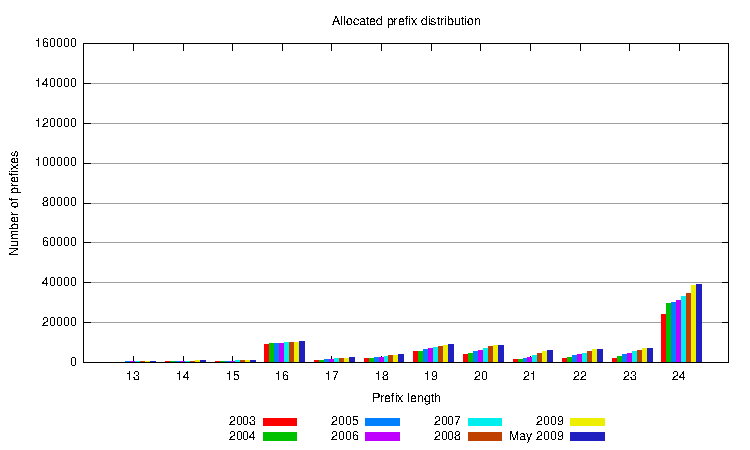
\includegraphics[width=0.5\textwidth]{02_prefixes/02_ip_prefixes_zoom}
	\caption{Allocated prefix distribution}
 	\label{fig:IP allocations}
\end{figure}
The distribution of allocated block sizes has changed over the past six years, as shown in figure \ref{fig:IP allocations}. The number of allocations has increased for every prefix prefix length, but at different rates. In 2003, /24 was the most popular size, as it is today, but there were only about half as many /20 allocations as /19 ones, whereas in 2008 they are about the same. There has been almost no increase in /16 blocks. Throughout the siz-year period, most IP allocations are /24 blocks. The next most popular block size is /16, followed by /19 and /20. The smaller block sizes (/19 and smaller) have had a larger increase in usage than /16, /17, and /18.
\subsection{Yearly distribution of IP allocations}
\begin{figure}[htbp]
 	\centering
 		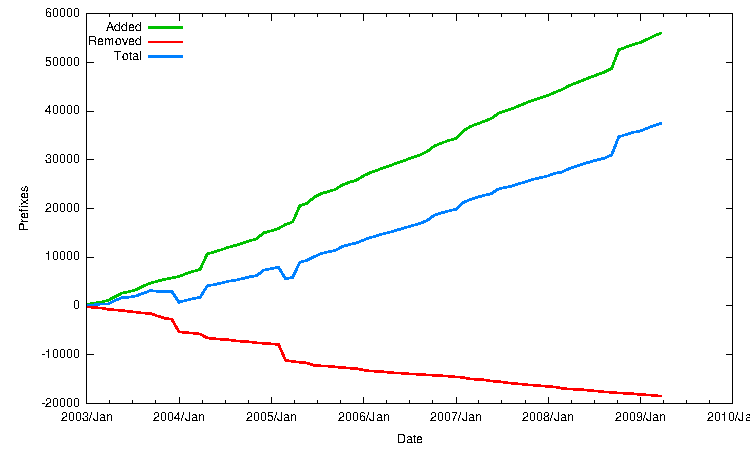
\includegraphics[width=0.5\textwidth]{04_plus_minus/addremoveprefixallocculmulative}
	\caption{Trends in IP prefix allocation}
 	\label{fig:IP allocations new and gone}
\end{figure}
Figure \ref{fig:IP allocations new and gone} shows that the number of allocated IP prefixes has increased by almost 40,000 in the past six years. Some allocations have disappeared, but a larger number of new allocations has outpaced the disappearances.

\subsection{Unaligned allocation}
Unaligned IP allocations are ones whose size is not a power of two. For instance, a block of 1000 addresses could be allocated instead of 1024. The latter could be represented by a single /22 prefix, whereas the former would need a /23, /24, /25, /26, /27, and /29 prefix to express the allocation. Allocations usually have size of a power of two, so a single prefix will suffice. There are not very many unaligned allocations because they are wasteful of BGP table space and have no advantages over aligned ones. Figure \ref{fig:unaligned IP allocations} shows the distribution of such allocations. Most were allocated between 1992 and 1995, although there have been some every year since then. Compared to the size of the entire routing table, these allocations are insignificant, but it is interesting that they exist at all, since RIRs should know better.
\begin{figure}[htbp]
 	\centering
 		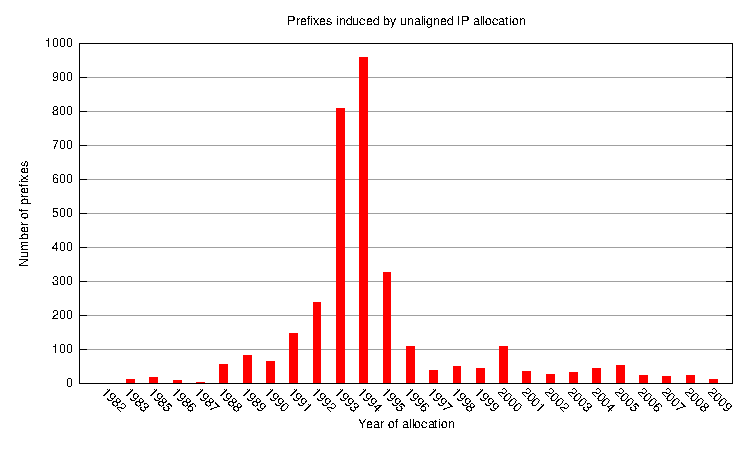
\includegraphics[width=0.5\textwidth]{09_alloc_adhoc/adhoc}
	\caption{Unaligned IP allocations per year}
 	\label{fig:unaligned IP allocations}
\end{figure}
\subsection{Allocation by geographical region}

\subsection{Allocation changes by geographical region}
\begin{figure}[htbp]
 	\centering
 		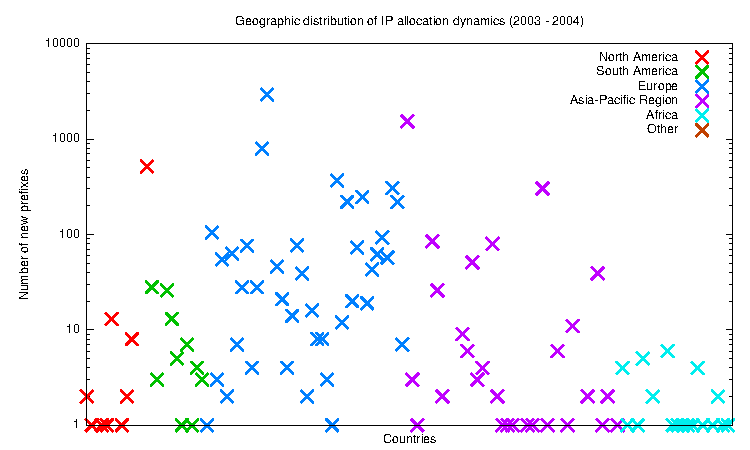
\includegraphics[width=0.5\textwidth]{04_2_plus_minus_countries/plus_minus_2003-01-01}
	\caption{Increase in allocations by region 2003}
 	\label{fig:increase2003}
\end{figure}
\begin{figure}[htbp]
 	\centering
 		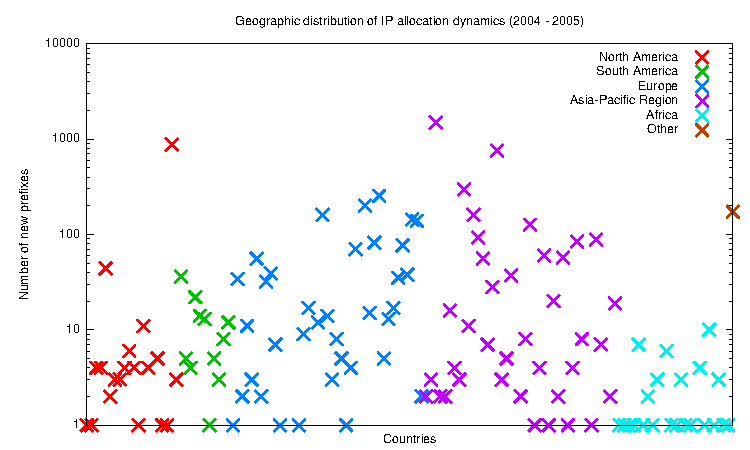
\includegraphics[width=0.5\textwidth]{04_2_plus_minus_countries/plus_minus_2004-01-01}
	\caption{Increase in allocations by region 2004}
 	\label{fig:increase2004}
\end{figure}
\begin{figure}[htbp]
 	\centering
 		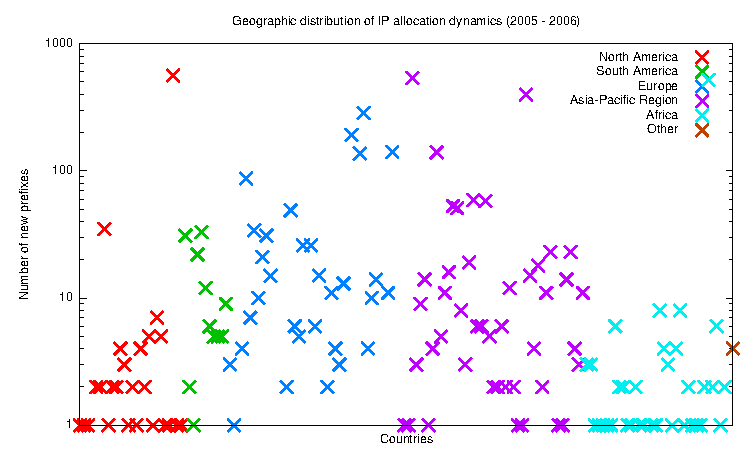
\includegraphics[width=0.5\textwidth]{04_2_plus_minus_countries/plus_minus_2005-01-01}
	\caption{Increase in allocations by region 2005}
 	\label{fig:increase2005}
\end{figure}
\begin{figure}[htbp]
 	\centering
 		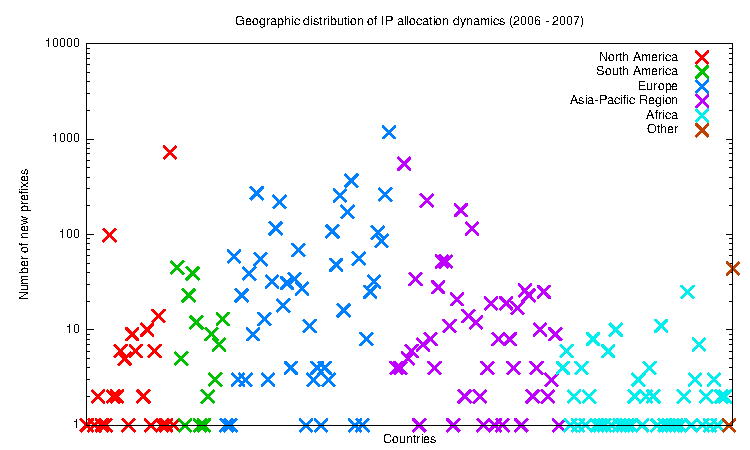
\includegraphics[width=0.5\textwidth]{04_2_plus_minus_countries/plus_minus_2006-01-01}
	\caption{Increase in allocations by region 2006}
 	\label{fig:increase2006}
\end{figure}
\begin{figure}[htbp]
 	\centering
 		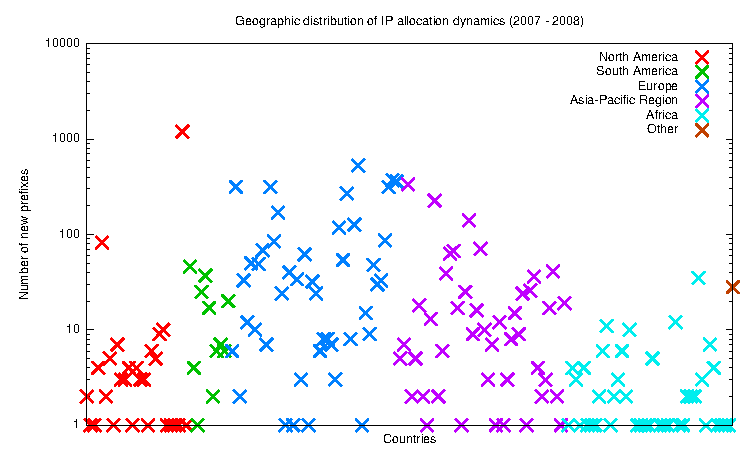
\includegraphics[width=0.5\textwidth]{04_2_plus_minus_countries/plus_minus_2007-01-01}
	\caption{Increase in allocations by region 2007}
 	\label{fig:increase2007}
\end{figure}
\begin{figure}[htbp]
 	\centering
 		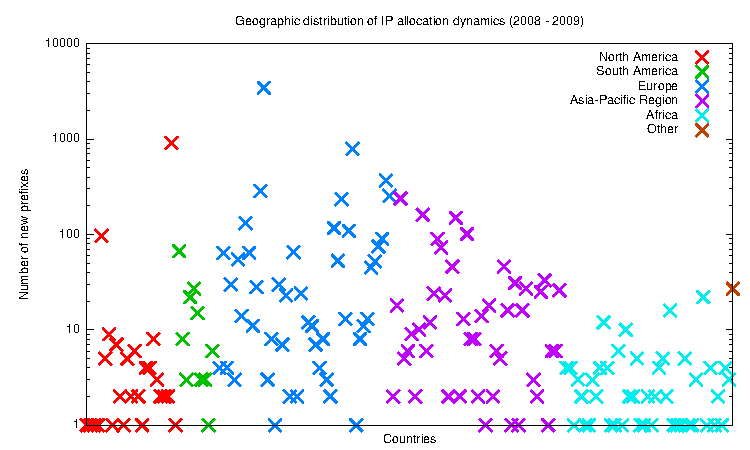
\includegraphics[width=0.5\textwidth]{04_2_plus_minus_countries/plus_minus_2008-01-01}
	\caption{Increase in allocations by region 2008}
 	\label{fig:increase2008}
\end{figure}
As can be seen in figures \ref{fig:increase2003}-\ref{fig:increase2008}, the increase in allocations each years has no clear trend and does not appear to vary in a consistent way. In each country in can vary significantly from one year to the next. The same countries do not allocated more than others every year. 